\documentclass[12pt, a4paper]{article}

\usepackage[spanish]{babel}
\usepackage{geometry} 
\usepackage{graphicx}     
\usepackage{float}
\geometry{margin=2.5cm}

\title{\textbf{Reporte LeetCodes}}
\author{García Rayón Dylan Osvaldo\\
Córdova García Diego\\
Robles de la Rosa Mauro Alexis}
\date{\today}

\begin{document}

\maketitle

\section{LeetCode 1011}
Dada una lista de los pesos de varios paquetes y una cantidad de días fija, hallar la capacidad mínima de carga para entregarlos todos.

\subsection{Resolución con Búsqueda Binaria}
El problema plantea determinar la capacidad mínima de carga de un barco para trnasportar un cojunto secuencial de paquetes en un límite de D días,
respetando estrictamente el orden original en el que se presentan.

El rango de capacidades posibles del barco está acotado de forma natural:

El límite inferior es el peso del paquete más pesado, ya que el barco debe ser capaz al menos de cargar el elemento individual de mayor masa.

El limite superior es la suma total de los pesos, que representa el escenario donde todos los paquetes se transportan en un solo día.

Existe una relación inversa, a mayor capacidad de carga, menor número de días necesarios para completar el envío; a menor capacidad, más días se requieren.
La invariante del algoritmo (Búsqueda Binaria) garantiza que evaluando un punto medio mediante una simulación lineal, se puede descartar de manera segura la mitad
del espacio de búsqueda hasta converger en la capacidad óptima mínima.

\subsection{Optimización}
Probar de manera secuencial cada capacidad entera desde los pesos máximos hasta la suma de los pesos tomaría un tiemppo proporcional al tamaño del rango total (O(Suma-Máximo))
lo cual es ineficiente si los pesos o la suma son grandes.

Al aplicar Búsqueda Binaria sobre el rango de capacidades, el espacio de búsqueda se reduce a la mitad en cada paso. Esto transforma un problema de optimización en uno de búsqueda
logarítmica, reduciendo drásticamente el número de evaluaciones de capacidad de lineal a logarítmica con respecto al valor numérico de la suma de pesos.

\subsection{Complejidad Temporal}
O(n log S), donde n es el número de paquetes en el arreglo y S es la diferencia entre la suma total de los pesos y el peso máximo.

\subsection{Complejidad Espacial}
O(1). El algoritmo opera exclusivamente utilizando variables primitivas de control para los apuntadores del rango (low, high, mid) y contadores locales durante la simulación de los días,
sin requerir estructuras de datos auxiliares ni memoria adicional.

\begin{figure}[H]
    \centering
    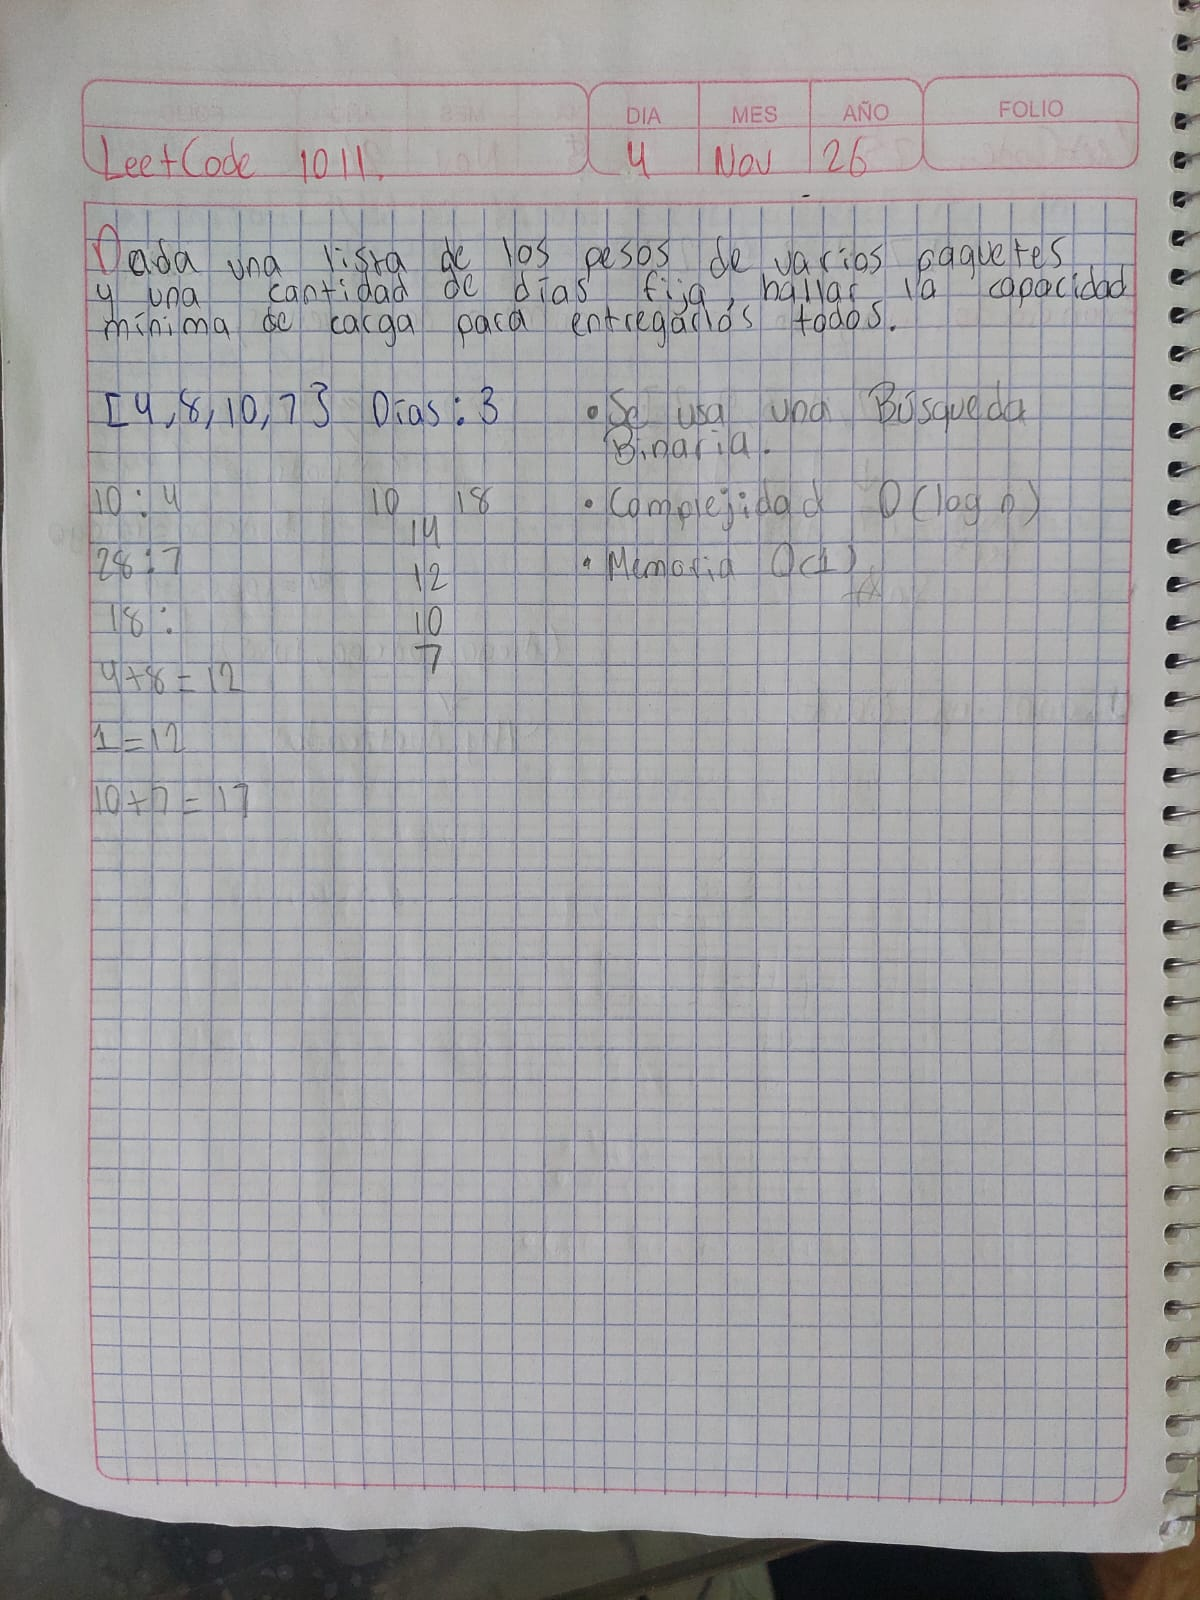
\includegraphics[width=0.6\textwidth]{imagenes_leetCodes/LC1011.jpeg}
    \caption{LeetCode 1011}
\end{figure}

\section{LeetCode 98}
Dada la raíz de un árbol binario determinar si es un árbol de búsqueda binario válido

\subsection{Resolución con Atravesamiento de árboles (Preorden)}
El problema consiste en determinar si un árbol binario dado es un Árbol Binario de Búsqueda (BST) válido. La condición fundamental de un BST dicta que para cualquier nodo, todos los valores 
en su subárbol izquierdo deben ser estrictamente menores que la clave del nodo, y todos los valores en su subárbol derecho deben ser estrictamente mayores.

Al recorrer el árbol en Preorden (visitando primero el nodo raíz y luego descendiendo hacía sus subárboles izq y der), la invariante clave que se propaga en cada llamada recursiva es un rango 
válido de valores permitidos.

Cuando se visita el nodo raíz, se valida inmediatamente si su valor se encuentra dentro de los límites actuales permitidos.

Al descender al subárbol izquierdo, el límite superior se actualiza al valor del nodo actual (ya que ningún descendiene izq puede ser mayor o igual al padre). Al descender al subárbol derecho, el límite
inferior se actualiza al valor del nodo actual.

\subsection{Optimización}
Un error común de fuerza bruta consiste en verificar únicamente que nodo.izq.val < nodo.val < nodo.der.val para cada nodo de forma aislada. Esto es incorrecto porque un nodo en un subárbol izquierdo profundo
podría violar la regla del BST con respecto a un ancestro superior (por ejemplo, ser mayor que la raíz del árbol).

Otra opción clásica es hacer un recorrido en orden y verificar que los elementos resultantes formen una secuencia estrictamente ascendente. Sin embargo, requiere almacenar o comparar el valor previo, mientras 
que el enfoque de Preorden con propagación de límites permite cortar la recursión de forma temprana tan pronto como se detecta una violación del rango, sin necesidad de recorrer todo el árbol 
si la condición falla en niveles superiores.

Con Preorden visita cada nodo exactamente una vez, aprovechando la pila de llamadas del sistema de manera óptima.

\subsection{Complejidad Temporal}
O(n), donde n es el número total de nodos en el árbol binario. En el peor de los casos, el algoritmo debe visitar cada nodo del árbol una sola vez para verificar y propagar los límites de validación, alcanzando una cota lineal 
estricta.

\subsection{Complejidad Espacial}
O(h), donde h es la altura del árbol binario.

\begin{figure}[H]
    \centering
    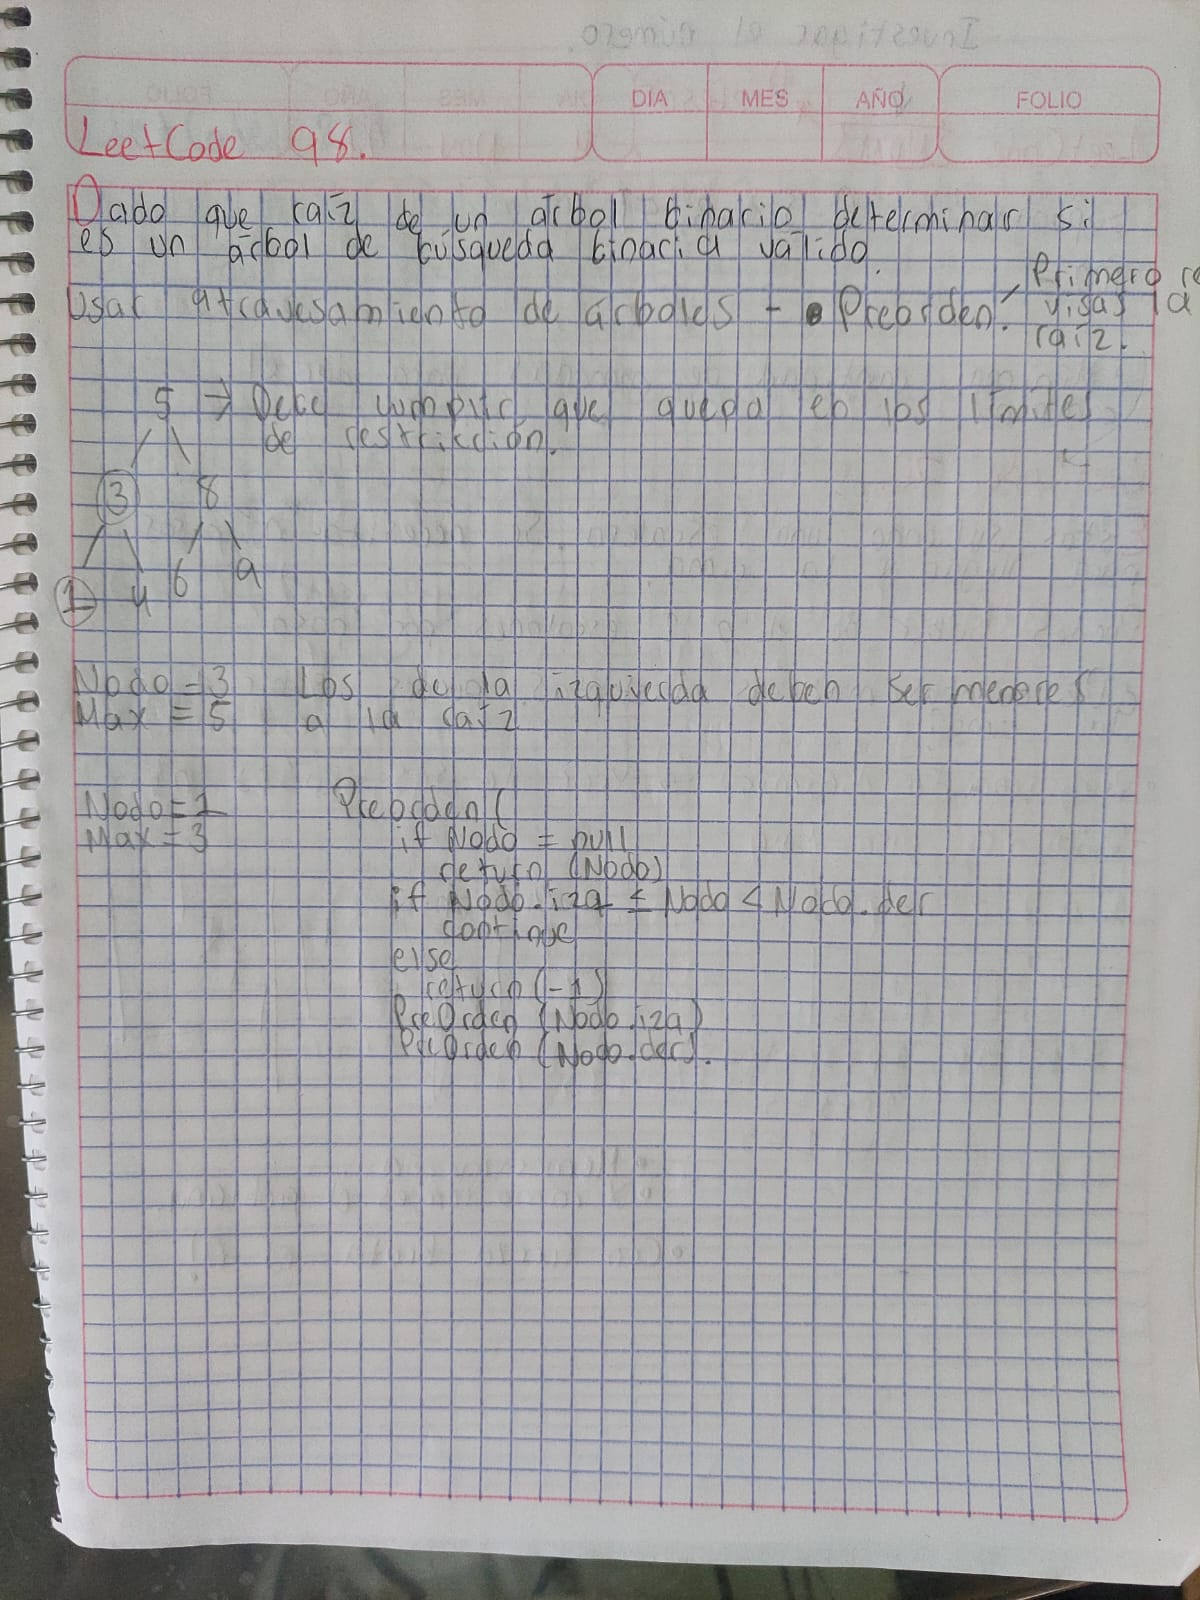
\includegraphics[width=0.6\textwidth]{imagenes_leetCodes/LC98.jpeg}
    \caption{LeetCode 98}
\end{figure}

\end{document}